%!TEX root = ../Technical_paper.tex
\section{Physiological structure of the human hand}
\label{sec:Physiological_structure_of_the_human_hand}
Lee and Kuni \cite{LEE.1995} described the human hand as "\textit{an articulated structure with about 30 degrees of freedom [which] changes shape in various ways by its joint movements.}"\\
All of the hand parts are connected to at least one neighboring part via a \textit{joint}. The \textit{joints} affect the position of the connected part. To describe the movement of the hand parts, we can use the rotation angles of the joints to correlate to a specific position.
To do so, we define a local coordinate system for each of the exiting hand joints. Through these coordinate Systems, we achieve a sequence of rotations in the local coordinate systems of the joints. Such a sequence can then be used to describe a specific movement and/or position of a part.
Not all of the joints in the human hand have equal \textit{degrees of freedom}. Their functionality can be classified in the amount of DOFs (\textit{degrees of freedom})\cite{KOREIN.1985} where 1DOF joints can perform a \textit{flexion} or \textit{twist} in one direction. The 2DOF joints can perform \textit{flexion} movement in more than one direction and the 3DOF joints can perform simultaneous simultaneous \textit{directive} and \textit{twist} movements.\\
Regarding the human hand, each finger sums up to 4 DOF's and the thumb to 5 DOF's. Also considering 6 DOFs for the rotation and position of the whole hand, the total sum add up to 27 DOFs.
\subsection{Constraints in hand motion}
\begin{figure}[ht]
\centering
	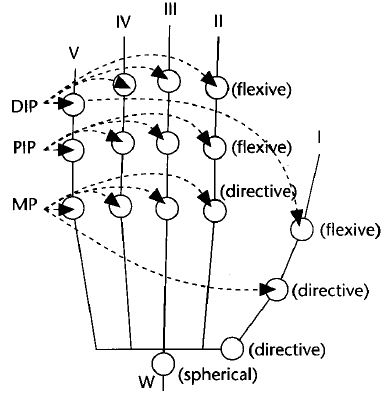
\includegraphics[width=\columnwidth/2]{images/Hand_DOFs.JPG}
	\label{Handstructure} 
	\caption{Joint constraints of the human hand (\cite{LEE.1995})}
\end{figure}
A full usage of all the declared DOFs would lead to a large amount of possible combinations. Since the hand is not only made up of bones but also muscles and the skin, we can impose some constraints \cite{Badler.1987,Pavlovic.1997} to the movement of the joints. Ling, Wu and Huang\cite{LIN.2000} proposed following classification for the constraints:
The \textbf{Type I} and \textbf{Type II} constraints rely on the physiological and mechanical properties of the human hand.\textbf{Type III} constraints are results of common and natural movements. Therefore these constraints will be differing form person to person. However, these movements are to a certain degree similar for everyone. Accordingly, a broad grouping can be applied. For the mathematical description of the \textbf{Type I} and \textbf{Type II} constraints,the following inequalities can be used:
\begin{equation}
\begin{split}
0\degree&\leq \Theta _{MP_{flex}} \leq 90\degree\\
0\degree&\leq \Theta _{PIP_{flex}} \leq 110\degree\\
0\degree&\leq \Theta _{DIP_{flex}} \leq 90\degree\\
-15\degree&\leq \Theta _{MP_{abduct/adduct}} \leq 15\degree
\end{split}
\end{equation}
\\For the middle finger, a further specific constraint is applicable as the middle fingers MP joint normally does not abduct and adduct much. Therefore an approximation is applicable, resulting in the removal of 1 DOF from the model:
\begin{equation}
\Theta _{MP_{abduct/adduct}}=0\degree
\end{equation}
The same behavior can be seen in the combination of hand parts labeled W( the connection point between hand and lower arm). This approximation also eliminates one DOF on the connected thumb:
\begin{equation}
\Theta _{W_{abduct/adduct}}=0\degree
\end{equation}
Since the DIP,PIP and MP joints of our index, middle, ring, and little fingers only have 1 DOF for flexion, we can further assume that their motion is limited to movement in one plane. \\\\
The \textbf{Type II} constraints can be split into \textit{inter-finger} and\textit{ intra-finger} constraints.
Regarding \textit{intra-finger} constraints between the joints of the same finger, human hand anatomy implies that to bend the DIP joints on the specific finger,the corresponding PIP joints of that finger must also be bent.
The approximation for this relation\cite{Rijpkema.1991} can be described as :
\begin{equation}
\Theta _{DIP} =\frac{2}{3}\Theta _{PIP}
\end{equation}
\textit{Inter-finger} constraints can be imposed between joints of adjacent fingers. \textit{Inter-finger} constraints describe that the bending of an MP joint in the index finger forces the MP joint in the middle finger to bend as well.\\
 When combining the constraints described in the above equations, the initital number 21 DOF's of the human hand can be reduced to 15. Inequalities for these cases, obtained through empiric studies, can be found in \cite{LEE.1995}.\\
\section{Kinematics}
\label{sec:kinematics}
Kinematic systems contain so called \textit{kinematic chains}, which consist of a \textit{starting point} or \textit{root}, kinematic elements like \textit{joints}, \textit{links} and an \textit{endpoint}, also called \textit{end effector}. Applied to the human hand, the whole hand model represents the kinematic system. This system contains several \textit{kinematic chains}, namely the fingers of the hand with the fingertips being the \textit{end effectors} of each of these chains.
\\Each of these components has it's set of DOF's which can be described mathematically. As hand movements starts, the states of the kinematic chains begin to change. Joint angles and end effector positions are modified until the end position is reached. To represent the new position and angle values of our physical hand with a kinematic system, two major paths for achieving a solution can be taken.\\\\
The Forward Kinematics(FK) approach uses the knowledge of the resulting angles and positions after the application of known transformations to the kinematic chain. The resulting new positions of the \textit{joints} and \textit{links} between the \textit{root} and the \textit{end effector} is used to solve the problem of finding the \textit{end effector's} position.\\
The advantage of an FK solution is that there is always an unique solution to the problem. In consequence, this approach is commonly used in the field of robotics, where the information on the chain elements is easily available.
The tracking of the human hand and all of its chain components is rather complicated. Therefore a solution which takes a known position of the \textit{end effector} and calculates the parameters for the rest of the chain is more desirable.\\
The concept of \textit{Inverse Kinematics}(IK) already describes it's principle in it's name. It takes the reversed approach in comparison to the FK principle. Instead of knowing the states of the chain elements and calculating the resulting position of the \textit{end effector}, we take the position of the \textit{end effector} and try to retrieve the possible states of the other chain elements. \\
In contrary to having a unique solution with the FK approach, the IK approach can end at the point of not finding a suitable solution.
Established solution for solving inverse kinematic problems mostly rely on matrix calculations. These methods include solving via Jacobian Inverse\cite{DavidE.Orin.1984,Wolovich.1984}, Jacobian transpose, Jacobian pseudo inverse\cite{Golub.1965,Dahmen.2008}, Damped Least Squares\cite{Wampler.1986,Nakamura.1986} and Newton Methods. All of these methods have a rather high computational load and some can suffer from singularities, making a solution not obtainable.
\\A more recent approach in the kinematics field is the \textit{FABRIK} algorithm proposed by Aristidou and Lasenby\cite{Aristidou.2011}.
The \textit{FABRIK} algorithm does not depend on these matrix operations as is solves for the position of a point on a line to retrieve the new joint positions. This is done in an forward and also inverse solving approach, iterating these steps until the calculated position converges towards the target position from the tracking data.
\\The chain joints are denoted as $\textbf{p}_{\textit{i}}$ with the distance $\textbf{d}_{i}$ being $|\textbf{p}_{\textit{i+1}}-\textbf{p}_{\textit{i}}|$. The target point for the end effector is denoted as \textbf{t}.The joint positions are taken from either a previous iteration or from an initial calibration. 
But before calculations can begin, the algorithm has to check whether the intended target point \textbf{t} is reachable for the end effector.This is done by measuring the distance between the root of the kinematic chain and the target point \textbf{t}. This value is then compared with the sum of the distances $\textbf{d}_{i}$.
\begin{equation}
 dist_{t,d_{1}}< \sum_{k=1}^{i}{d_{i}}
\end{equation}
If the summed distance is greater, then the target \textbf{t} is within the reach of the system and the calculation can continue, otherwise the calculation has to be aborted and the error has to be manged otherwise.
Assuming this requirement to be met, we can now begin with the first calculation.The inverse calculation step is the first step.The calculation is started at the end effector, moving to the root of the chain.  Therefore we assume that the new position $\textbf{p}_{n}^{'}$ with n=4,...,1 is equal to \textbf{t}.
\begin{equation}
 \textbf{p}_{n}^{'}=\textbf{t}
\end{equation}
\\From this new point, we can construct a line that goes through $\textbf{p}_{n}^{'}$ and $\textbf{p}_{n-1}$.
\begin{equation}
\begin{split}
A&=\textbf{p}_{n}^{'}\\
B&=\textbf{p}_{n-1}\\
\textbf{l}_{n-1}&=\overline{AB}\\
\end{split}
\end{equation}
\\The resulting position of the new $\textbf{p}_{n-1}^{'}$ point is located on this line with the distance of $\textbf{d}_{n-1}$ from $\textbf{p}_{n}^{'}$ (see \textbf{(c)}).\\
\begin{equation}
\textbf{p}_{n-1}^{'}= \textbf{p}_{n}^{'}+ \left(\frac{\overline{AB}}{|\overline{AB}|}\cdot\textbf{d}_{n-1}\right)
\end{equation}
Consecutively, this is done with the remaining joints until the root joint is reached.
This finishes the first halve of the iteration step.With the calculated positions, we now perform a forward calculation, starting from the root until we reach the end effector. Since the root of the system normally does not move from it's initial position, we have to reset the root joint to this value before starting to calculate the new positions of the subsequent joints(see\textbf{(e)}).

Analogous to the procedure in the inverse step, we construct the lines between the points and determine the new position values of the joints. At this point, we can decide if the result position of the end effector is appropriate in comparison to the value of \textbf{t}. A simple threshold value for this case could be the position difference between these two points.
\\Since this algorithm does not rely on the heavy-weight calculation operations, it converges much faster and in less iterations. Furthermore the incorporation of constraints to the calculation does not interfere with this values and is rather easy.